% Document class & environment definition -----------------------------------------------
\documentclass[11pt]{book}

\usepackage[utf8]{inputenc}

\usepackage[english]{babel}

\usepackage[T1]{fontenc}

\usepackage{setspace}

\usepackage{amsfonts}

\usepackage{harmony}

\usepackage{graphicx}
\graphicspath{ {./images/} }

\usepackage{geometry}
\geometry{a4paper, top=3cm, bottom=3cm, left=3cm, right=3cm}

\usepackage{amsmath}
\numberwithin{section}{chapter}
\numberwithin{equation}{subsection}
\numberwithin{figure}{chapter}

\usepackage[a-2b,mathxmp]{pdfx}
\usepackage[pdfa]{hyperref}

\usepackage{xcolor}
\usepackage{color}

\usepackage{fancyhdr}
\pagestyle{fancy}
\lhead{}
\chead{}
\rhead{}
\lfoot{Consorzio RFX - Ricerca Formaxzione Innovazione}
\cfoot{}
\rfoot{\thepage}

\usepackage{subcaption}


% Commands ------------------------------------------------------------------------------
\newcommand{\Cels}{^{\circ}C}
\newcommand{\half}{\frac{1}{2}}
\renewcommand\thesection{\arabic{section}}
\renewcommand{\headrulewidth}{0.5pt}
\renewcommand{\footrulewidth}{0.5pt}


\begin{document}
	
	\begin{titlepage}
		\begin{center}
			
\includegraphics[width=0.5\textwidth]{images/rfx_logo.png}
			\vspace{1.5cm}
			\Huge 
			\doublespacing 
			\bfseries 
			\begin{spacing}{1}
				\textsc{Getting started with the KRIA KR260 Robotics Starter Kit}
			\end{spacing}
			\vspace{0.5cm}
			\textsc{\large A simple example project}
			\vfill
			\small 
			Author : Bevilacqua Mattia\\
			Date : Dec. 2024 
		\end{center}
	\end{titlepage}
	
	\clearpage
	\null
	\thispagestyle{empty}
	\clearpage
	
	\chapter*{Preface}
The aim of this guide is to give a reference design flow for the creation of a project using both Vivado and Petalinux SDK. Within this way of programming, the bare metal approach, such as the one normally used for STM micro controllers, gives more space to a OS-oriented method. To all intents and purposes, after the creation of the project, what is left is a tailor-made OS that will manage the board in a similar way to that of the bare metal, but with all the advantages of having a OS.
\bigskip
\\Even though some passages are explained, it is given for granted that the developer has some basic knowledge of the Vivado and Petalinux environments. While a the creation of the Vivado- Petalinux project and further implementations are illustrated, it is left for the reader to find a way to create the environment needed to follow the steps disclosed in the following. To write this document and to create the project the following software/devices have been used:
\begin{itemize}
	\item Kria KR260 Robotic Starter Kit
	\item Vivado 2024.1
	\item Petaliux SDK v2022.2
	\item CenOS stream 9
\end{itemize}
Newest software releases might not be compatible with the procedure(s) listed and/or with the files used to support the processes. It is recommended to check resources availability and compatibility before the installation of Vivado and, paying more attention, of Petalinux SDK.
\bigskip
\\The guide is divided into four chapters. The first chapter gives an overview of the Petalinux installation procedure with the bespoke OS (Operative System). The second chapter deals with the creation of a simple project that will exploit the programmable logic (PL). This method is called bare-metal programming. The third chapter proposes the same project under a new light: the creation of a bootable SD card and the running of the project from within the SD card. The last chapter deals with the creation of a PS application so as to read a register. At the end of each project there is also a debugging session utilizing the J-TAG interface.
	
	\clearpage
	\null
	\thispagestyle{empty}
	\clearpage
	
	\tableofcontents
	
	\clearpage
	\null
	\thispagestyle{empty}
	\clearpage
	
	\chapter{Petalinux} \label{ch:petalinux}
Petalinux is an embedded Software Development Kit - SDK - targeting FPGA-based System on a Chip - SoC - design or FPGA designs.


\section{Installation procedure}
Before the actual installation of Petalinux SDK, the creation of a compatible environment is requested.
There are few steps to be followed in order to configure such environment:
\begin{itemize}
	\item Adding the 32-bit architecture to the system
	\item Installing all the required packages for the Petalinux Build Host 
\end{itemize}

\subsection{i386 architecture}
The 32bit architecture is essential for Petalinux to be installed. To add such architecture to the system, open the command prompt and type the following command:
\begin{verbatim}
	$ sudo dpkg --add-architecture i386
\end{verbatim}
It is now possible to check the availability of the architecture by typing
\begin{verbatim}
	$ dpkg --print-foreign-architectures
\end{verbatim}
and an output similar to that of Figure \ref{fig:i386} will appear.
\begin{figure}[ht]
	\centering
	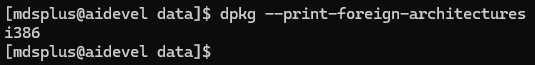
\includegraphics[width=0.7\textwidth]{images/i386}
	\caption{Successful installation of i386 architecture.}
	\label{fig:i386}
\end{figure}

\subsection{Petalinux Build Host packages}
From this \href{https://adaptivesupport.amd.com/s/article/73296?language=en_US}{page}, download the file at the bottom. Create the folder in which petalinux will be installed with the command \begin{verbatim}
	mkdir <folder_name>
\end{verbatim}
and copy the file from the download folder to the this final folder. Within this example, such folder is named ptlnx. To start the installation of all the packages type 
\begin{verbatim}
	chmod +x <installer_file_name>
	sudo ./<file_name>
\end{verbatim}
Once the installation is complete, all the packages should have been installed.

\subsection{Petalinux SDK installation}
Now it is possible to begin the actual installation of Petalinux. From the \href{https://www.xilinx.com/support/download/index.html/content/xilinx/en/downloadNav/embedded-design-tools/archive.html}{AMD download page}, download the needed version and move it to the installation folder. From this page also download the .BPS file relative to the board to be used. This latter file has to be moved into the folder in which the petalinux project are saved. Now type
\begin{verbatim}
	chmod +x <installer_file_name>
	./<file_name>
\end{verbatim}
Now the installation should begin. By following the instruction, the installation process should proceed without any inconvenience, even though it might take a while. Finally, to set the Petalinux environment into the directory in which it is installed, type
\begin{verbatim}
	source settings.sh
\end{verbatim}
from which the shell output is highlighted in Fig. \ref{fig:pt1} is shown. Now the system should be all set.
\begin{figure}[ht]
	\centering
	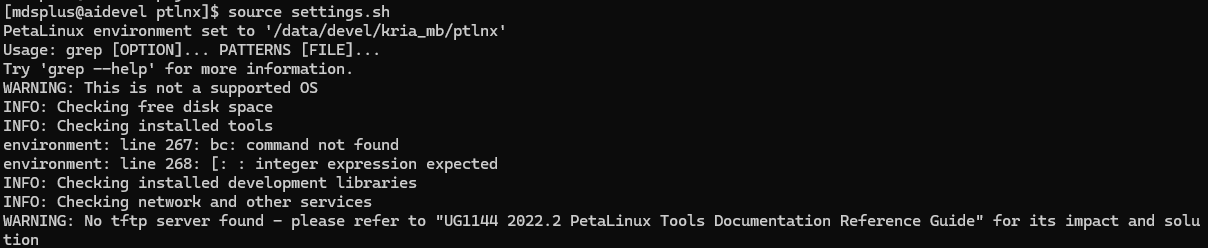
\includegraphics[width=\textwidth]{images/pt1}
	\caption{Setting petalinux environment.}
	\label{fig:pt1}
\end{figure}

	\chapter{Project 1: NAND gate - bare metal approach} \label{ch:nand_bm}
Within this chapter I+it will be explained how to program a FPGA, in this specific case the one mounted on the KR260 starter kit, with the so-called bare metal approach.


\section{Vivado project}
Vivado is a software developed by AMD which is oriented to programming Field Programmable Logic Arrays - FPGAs - which supports various board and modules. It is a free software, even though an account is requested for the download(s).
\bigskip
\\The example project that will be discussed within this chapter is meant only to give an introduction to the Vivado-FPGA programming world, which is way more vast and deeper. The description is quite simple: a simple NAND gate which controls a user defined LED mounted on the development board.
\begin{figure}[ht]
	\centering
	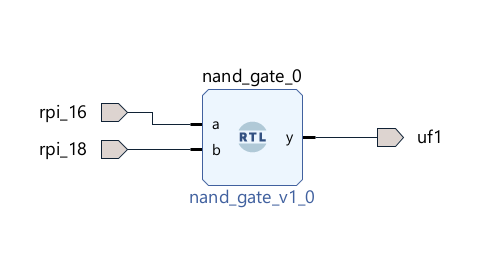
\includegraphics[width=0.65\textwidth]{images/prj1_1}
	\caption{NAND gate Vivado block design.}
	\label{fig:prj1_1}
\end{figure}
As it can be see the implementation is quite trivial, consisting only of one module, which is the behavioral description of the NAND gate.

\subsection{Project creation}
Once Vivado is open and the start page loaded, create a new project named \textbf{nand\_bm} (or whatever other name) and skip directly to the board selection window. In this window, select the name of the development board it is about to be used and create the project. The first two tasks to carry out are NAND gate behavioral description file creation and the physical constraint constraints definition.

\subsection{Behavioral description}
Move to \textbf{Sources} $\rightarrow$ \textbf{Design Sources} $\rightarrow$ right-click on this latter one $\rightarrow$ \textbf{Add Sources}. A window like the one shown in Figure \ref{fig:prj1_2} should appear.
\begin{figure}[ht]
	\centering
	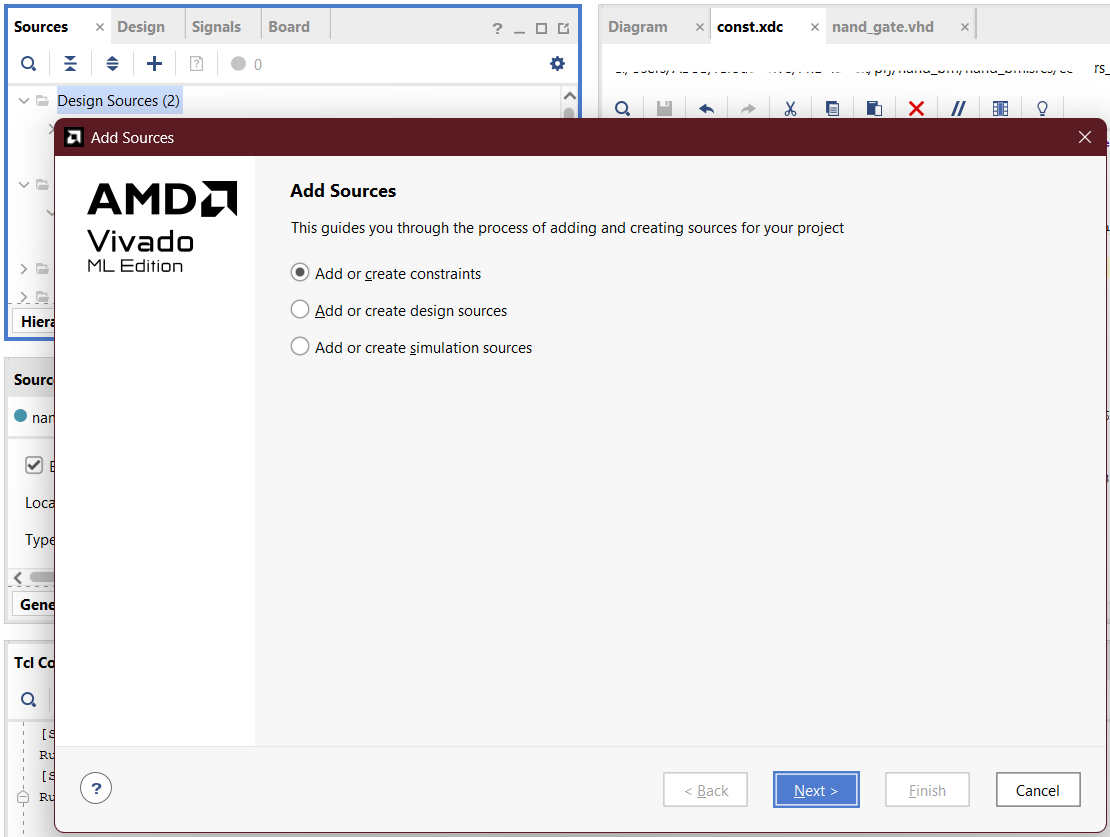
\includegraphics[width=\textwidth]{images/prj1_2}
	\caption{Add Sources window.}
	\label{fig:prj1_2}
\end{figure}
Select \textbf{Add or create design sources} $\rightarrow$ \textbf{Next} $\rightarrow$ \textbf{Create file} $\rightarrow$ enter the file name (nand\_gate) $\rightarrow$ \textbf{Finish}. Once it is done, a window to configure the inputs and the outputs of the gate should open. Such procedure can be skipped, providing that those information are defined in the description. The code to write down is the following:
\begin{verbatim}
	library IEEE;
	use IEEE.STD_LOGIC_1164.ALL;
	
	entity nand_gate is
	    Port ( a, b : in STD_LOGIC;
	              y : out STD_LOGIC);
	end nand_gate;
	
	architecture Behavioral of nand_gate is
	begin    
	    y <= a nand b;
	end Behavioral;
\end{verbatim} 
The project now has to be saved.

\subsection{Physical constraints}
The physical constraint file is the file that dictate which pin is connect to which within the development board and it of crucial importance for a real life application. Following a procedure similar to the one described for the behavioral description (\textbf{Sources} $\rightarrow$ \textbf{Constraints} $\rightarrow$ right-click on this latter one $\rightarrow$ \textbf{Add Sources} $\rightarrow$ \textbf{Add or create constraints} $\rightarrow$ \textbf{Next} $\rightarrow$ \textbf{Create file} $\rightarrow$ enter the file name (const) $\rightarrow$ \textbf{Finish}), the code to be written down is:
\begin{verbatim}
	set_property BITSTREAM.GENERAL.COMPRESS TRUE [current_design]
	
	#User defined pins
	set_property PACKAGE_PIN F8 [get_ports {uf1}]
	set_property IOSTANDARD LVCMOS18 [get_ports {uf1}]
	
	set_property PACKAGE_PIN AA12 [get_ports {rpi_16}]
	set_property IOSTANDARD LVCMOS33 [get_ports {rpi_16}]
	
	set_property PACKAGE_PIN Y9 [get_ports {rpi_18}]
	set_property IOSTANDARD LVCMOS33 [get_ports {rpi_18}]
\end{verbatim}
A bit of description it is needed to understand what those few lines of code do. The first line dictate that the bitstream that will be generated for this project will be compressed. The other lines define the port at which the buttons and the LED are connected (those information are provided from the datasheet of the board). For example, the pin at which the LED is connected is defined as a \textbf{standard I/O} with a voltage logic of \textbf{1.8V (LVCMOS18)}. In a similar way, the other two pins have the same characteristics, but with a voltage logic of \textbf{3.3V (LVCMOS33)}.

\subsection{Design generation}
Under the section of \textbf{IP INTEGRATOR}, click on \textbf{Create Block Design}: a new window will open. Move back to \textbf{Design Sources} $\rightarrow$ right click on the description file created earlier $\rightarrow$ \textbf{Add Module to Block Design}. To create a physical connection to the board pins, move the mouse tip on the block pins and type \textbf{Ctrl+T} to add a connection. By clicking on the created pins, a window named \textbf{External Port Properties} should appear. Rename those pins with the name define in the constraints file. Now the design should look like the one of Figure \ref{fig:prj1_1}

\subsection{FPGA programming}
To program the FPGA is needed a file that can be compared to the .hex file that will be generated for the programming of the a microcontroller (ATmega, STM32, ...). Move to the \textbf{PROGRAM AND DEBUG} section and click on \textbf{Generate Bitstream}. Follow the procedure and let the bitstream to be generated. The last step is to effectively program the device. Open the \textbf{Open Hardware Manager} and click on \textbf{Open Target} $\rightarrow$ \textbf{Auto Connect}, then click on \textbf{Program Device}.
	\chapter{Project 2: NAND gate}  \label{ch:nand}
Once one grasp the basic procedure to program an FPGA, by natural extension it should be asked how it is possible to exploit the full power of the SoM. This chapter offers a good start point, but it is just the tip of the iceberg. 
 



\section{Vivado project}
The project itself isn't changed: there is always the NAND gate. The only thing that is further added is the ability to boot the KR260 starter kit and to connect to it through the J-TAG interface. However, easy as it may seem, the procedure to follow is quite delicate and there are a lot of things to be taken care of.  The project will further analyze two ways of programming the FPGA: a) from within the SoM OS and b) at the boot of the board.
\begin{figure}[ht]
	\centering
	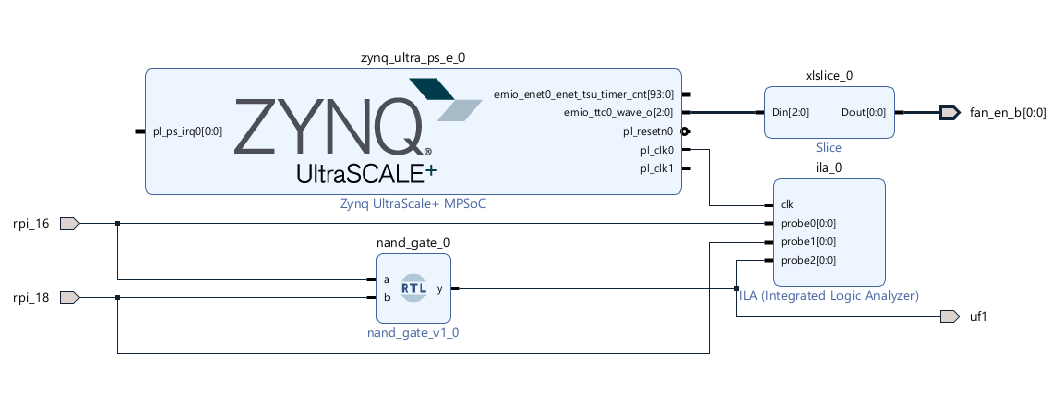
\includegraphics[width=\textwidth]{images/prj2_1}
	\caption{NAND gate Vivado block design.}
	\label{fig:prj2_1}
\end{figure}
Apart from the NAND design blobk, the project has been created from an example project given by AMD (this will include both the Zynq UltraScale+ MPsoC and the Slice). The ILA (Integrated Logic Analyzer) block serves the purpose to allow the view of the interesting waveform of the implementation during the debugging.
\bigskip
\\To create the project, open the Vivado main page, click on \textbf{Open Example Project} $\rightarrow$ \textbf{Next} $\rightarrow$ \textbf{Kria Starter Kit Design Example} $\rightarrow$ select the KR260 board $\rightarrow$ rename the project $\rightarrow$ \textbf{Default Bitstream} $\rightarrow$ create the project. To include both the source code of the NAND, follow the procedure explained in the previous chapter. The constrain file already exist, but it needs to be modified, adding the lines of code of the precious file. Once it is done, the file should look like in the following.
\begin{verbatim}
set_property BITSTREAM.GENERAL.COMPRESS TRUE [current_design]

#Fan Speed Enable
set_property PACKAGE_PIN A12 [get_ports {fan_en_b}]
set_property IOSTANDARD LVCMOS33 [get_ports {fan_en_b}]
set_property SLEW SLOW [get_ports {fan_en_b}]
set_property DRIVE 4 [get_ports {fan_en_b}]

#User defined pins
set_property PACKAGE_PIN F8 [get_ports {uf1}]
set_property IOSTANDARD LVCMOS18 [get_ports {uf1}]

set_property PACKAGE_PIN AA12 [get_ports {rpi_16}]
set_property IOSTANDARD LVCMOS33 [get_ports {rpi_16}]

set_property PACKAGE_PIN Y9 [get_ports {rpi_18}]
set_property IOSTANDARD LVCMOS33 [get_ports {rpi_18}]
\end{verbatim}
Open the design under the \textbf{IP INEGRATOR} section, add the NAND and the ILA blocks and connect them as it is showed in Figure \ref{fig:prj2_1}. Run both \textbf{Connection Automation} and \textbf{Block Automation} and let Vivado manage all the other connection. If needed, remake the wanted connections. Now, following the same procedure defined earlier, connect the I/O pins to the physical pins. The project should now be ready. 
To generate the wrapper, save the design and click on \textbf{Create HDL wrapper}. Make the new wrapper the top file (right click on the wrapper just created $\rightarrow$ \textbf{Make Top File}), generate the bistream, then move to \textbf{File} $\rightarrow$ \textbf{Export} $\rightarrow$ \textbf{Export Hardware} $\rightarrow$ \textbf{Include Bitstream}. The project is all set and it is now possible to focus on the Petalinux part.




\section{Petalinux project}
From within the Petalinux installation folder, type
\begin{verbatim}
	source ./settings.sh
\end{verbatim}
so as to set the Petalinux environment. Create now the project with the command
\begin{verbatim}
	petalinux-create --type project -s <path_to_bsp_file> --name <project_name>
\end{verbatim}
and once it is done, move into the folder just created. The following two steps are quite important, so it is recommended a bit more of attention.


\subsection{Base configuration}
The first configuration procedure aims to configure the core of the OS, i.e. to which architecture is addressed and which features are to be enabled. With the command
\begin{verbatim}
	petalinux-config --get-hw-description <path_to_xsa_file>
\end{verbatim}
a menu window will open (see Figure \ref{fig:prj2_2}), from which, moving into the various directories, the following packages must be enabled (or disabled):
\begin{itemize}
	\item \textbf{FPGA Manager} $\rightarrow$ \textbf{[*]FPGA Manager}
	\item \textbf{Image Packing Configuration} $\rightarrow$ \textbf{[]Copy final images to tftpboot}
\end{itemize}
\begin{figure}[ht]
	\centering
	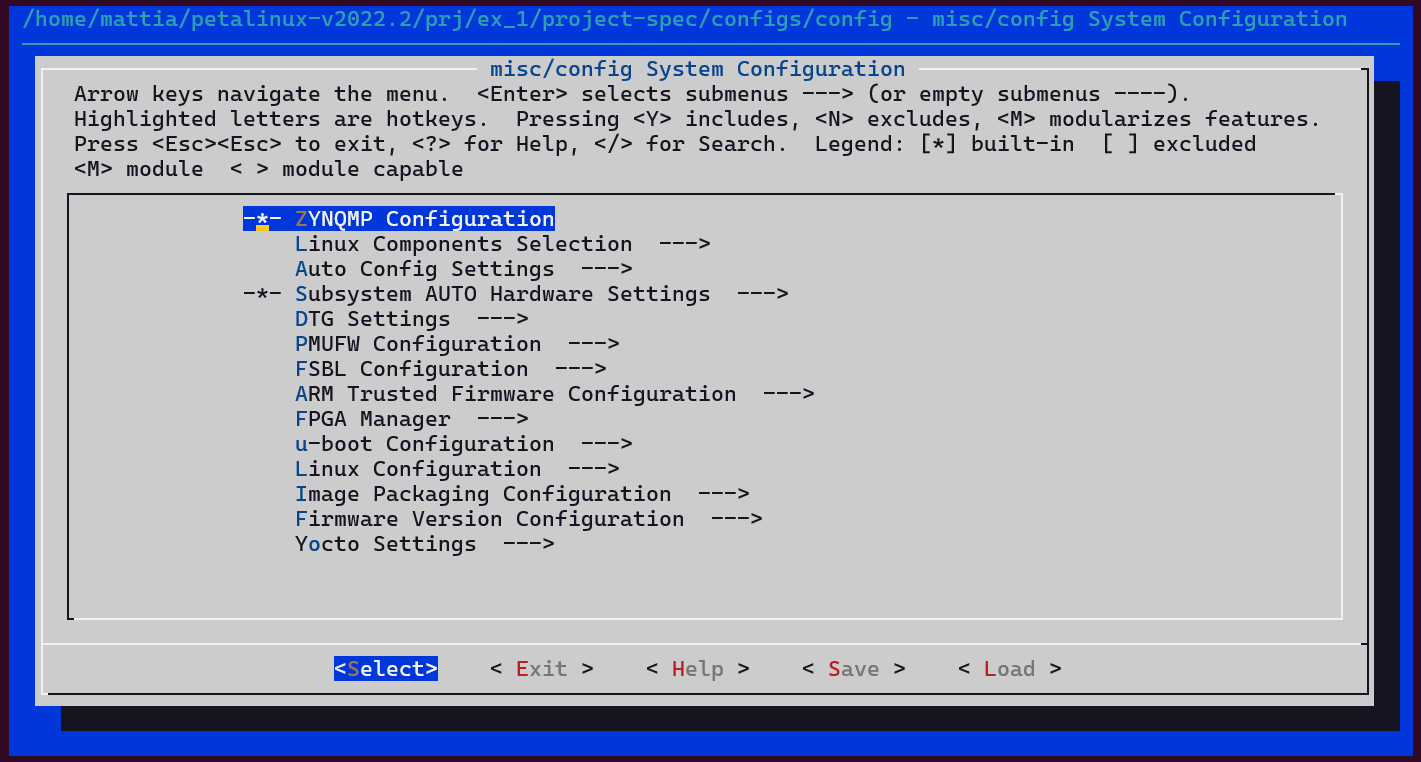
\includegraphics[width=\textwidth]{images/prj2_2}
	\caption{Base configuration window.}
	\label{fig:prj2_2}
\end{figure}
The FPGA manager will allow the FPGA to be programmed even during the operation of the board with few commands. However, it will generate an warning message during the creation of the BOOT.bin file.


\subsection{rootfs configuration}
The system to be created, in order to work, has to have some packages included, such as \textbf{bootget}, \textbf{gcc}, \textbf{XRT} and acceleration. The installation menu will open with the command
\begin{verbatim}
	petalinux-config -c rootfs
\end{verbatim}
from which the following packages have to be installed:
\begin{itemize}
	\item \textbf{Filesystem Packages} $\rightarrow$ \textbf{console} $\rightarrow$ \textbf{utils} $\rightarrow$ \textbf{git} $\rightarrow$ \textbf{[*]git}
	
	\item \textbf{Filesystem Packages} $\rightarrow$ \textbf{base} $\rightarrow$ \textbf{dnf} $\rightarrow$ \textbf{[*]dnf}
	
	\item \textbf{Filesystem Packages} $\rightarrow$ \textbf{x11} $\rightarrow$ \textbf{base} $\rightarrow$ \textbf{libdrm} $\rightarrow$ \textbf{[*]libdrm}, \textbf{[*]libdrm-tests}, \textbf{[*]libdrm-kms}
	
	\item \textbf{Filesystem Packages} $\rightarrow$ \textbf{libs} $\rightarrow$ \textbf{xrt} $\rightarrow$ \textbf{[*]xrt}, \textbf{[*]xrt-dev}
	
	\item \textbf{Filesystem Packages} $\rightarrow$ \textbf{libs} $\rightarrow$ \textbf{zocl} $\rightarrow$ \textbf{[*]zocl}
	
	\item \textbf{Filesystem Packages} $\rightarrow$ \textbf{libs} $\rightarrow$ \textbf{opencl-headers} $\rightarrow$ \textbf{[*]opencl-headers}
	
	\item \textbf{Filesystem Packages} $\rightarrow$ \textbf{libs} $\rightarrow$ \textbf{opencl-clhpp} $\rightarrow$ \textbf{[*]opencl-clhpp},\\ \textbf{[*]opencl-clhpp-dev}
	
	\item \textbf{Filesystem Packages} $\rightarrow$ \textbf{bootgen} $\rightarrow$ \textbf{[*]bootgen}, \textbf{[*]bootgen-dev}
	
	\item \textbf{Filesystem Packages} $\rightarrow$ \textbf{misc} $\rightarrow$ \textbf{packagegroup-core-buildessential} $\rightarrow$\\ \textbf{[*]packagegroup-core-buildessential},\\ \textbf{[*]packagegroup-core-buildessential-dev}
	
	\item \textbf{Filesystem Packages} $\rightarrow$ \textbf{misc} $\rightarrow$ \textbf{gcc-runtime} $\rightarrow$ \textbf{[*]libstdc++}, \\ \textbf{[*]libstdc++-dev}
	
	\item \textbf{Filesystem Packages} $\rightarrow$ \textbf{misc} $\rightarrow$ \textbf{gcr} $\rightarrow$ \textbf{[*]gcr}, \textbf{[*]gcr-dev}
	
	\item \textbf{Filesystem Packages} $\rightarrow$ \textbf{misc} $\rightarrow$ \textbf{gcr} $\rightarrow$ \textbf{[*]gdb}, \textbf{[*]gdb-dev}
	
	\item \textbf{Filesystem Packages} $\rightarrow$ \textbf{misc} $\rightarrow$ \textbf{glib-2.0} $\rightarrow$ \textbf{[*]glib-2.0}, \textbf{[*]glib-2.0-dev}
	
	\item \textbf{Filesystem Packages} $\rightarrow$ \textbf{misc} $\rightarrow$ \textbf{glibc} $\rightarrow$ \textbf{[*]glibc}, \textbf{[*]glibc-dev}, \textbf{[*]ldd}
	
	\item \textbf{Petaliunx Package Groups} $\rightarrow$ \textbf{packagegroup-petalinux} $\rightarrow$ \\ \textbf{[*]packagegroup-petalinux}
	
	\item \textbf{Petaliunx Package Groups} $\rightarrow$ \textbf{packagegroup-petalinux-gstreamer} $\rightarrow$\\ \textbf{[*]packagegroup-petalinux-gstreamer}
	
	\item \textbf{Petaliunx Package Groups} $\rightarrow$ \textbf{packagegroup-petalinux-opencv} $\rightarrow$\\ \textbf{[*]packagegroup-petalinux-opencv}
	
	\item \textbf{Petaliunx Package Groups} $\rightarrow$ \textbf{packagegroup-petalinux-v4lutils} $\rightarrow$\\ \textbf{[*]packagegroup-petalinux-v4lutils}
	
	\item \textbf{Petaliunx Package Groups} $\rightarrow$ \textbf{packagegroup-petalinux-x11} $\rightarrow$\\ \textbf{[*]packagegroup-petalinux-x11}
\end{itemize}
After this boring procedure, it is time to build the project with the command
\begin{verbatim}
	petalinux-build
\end{verbatim}
In the case of building failure with error messages not related to the implementation, try to clear out the current files by typing
\begin{verbatim}
	petalinux-config -x mr proper
\end{verbatim}
command which is used to deep cleaning the workspace, similar to how it's used in the Linux kernel build system.
\begin{figure}[ht]
	\centering
	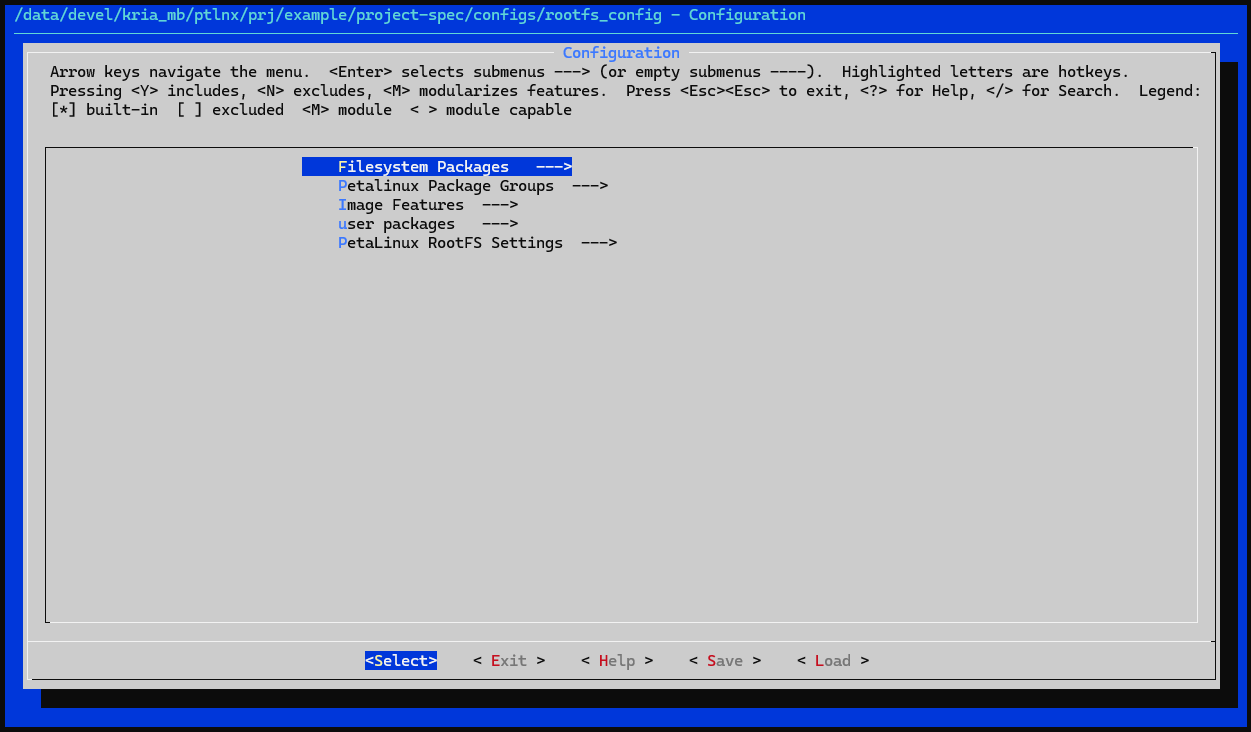
\includegraphics[width=\textwidth]{images/prj2_3}
	\caption{rootfs configuration window.}
	\label{fig:prj2_3}
\end{figure}


\subsection{Booting the board}
Since the board boots from a SD card, the system configuration just created has to be converted into a bootable image for the card. First step to carry out is the creation of the BOOT.bin file, which is of quite importance. To do so, after the project build, the command line is (on the same line)
\begin{verbatim}
	petalinux-package --boot --fsbl <path_to_elf_file> --fpga <path_to_bitstream>
	--u-boot
\end{verbatim}
in which the .elf file is usually located under the path images/linux/. The second step is to create a .wic image for the SD card to be flashed in. The command to do that is (on the same line)
\begin{verbatim}
	petalinux-package --wic --images-dir images/linux/ --bootfiles
	"ramdisk.cpio.gz.u-boot,boot.scr,Image,system.dtb,system-zynqmp-sck-kr-g
	-revB.dtb" --disk-name "sda"
\end{verbatim}
from which the .wic image will be generated and found in the same folder as the .elf file. To flash the SD card make use of a third-part software, such as balenaEtcher or something similar. Once the flash is done, insert the SD in the board and power it up. With a third part software, such as PuTTY, connect to the serial port (Baud Rate 115200). The system will require to inset some credential and the following may be used:
\begin{verbatim}
	ligin : petalinux
	password : your_password
\end{verbatim}
and now everything is set. To check if the packages are actually installed, type in the serial terminal
\begin{verbatim}
	gcc --version
	bootgen
\end{verbatim}
and some messages relating to the version or how to use them will be displayed.




\section{Programming the FPGA}
So far, only the boot was done with the procedure defined. The FPGA is not actually programmed. To do so, two ways can be used: the On-Run programming and the Boot programming. The first one allows for more flexibility and has the advantage to let the FPGA to be programmed even when the system is running, without the need to repeat all the steps previously explained. The second, thought being more rigid, allows for the FPGA to be programmed each time the system boots up. Within this example, the first approach has been chosen. To actually program the FPGA in after the system is booted, there is the need to convert the bitstream into a .bin file and then "manually" load it into the FPGA through the FPGA manager. Both .bit and the .bif file are to be copied in the SD card into an accessible folder. The .bif file has the following command lines:
\begin{verbatim}
	all:
	{
	    bit_file_name.bit
	}
\end{verbatim}
and through that the .bin file can be created using the command
\begin{verbatim}
	sudo bootgen -image <bif_file> -arch zynqmp -process_bitstream bin
\end{verbatim}
Now the .bin file has to be copied into the folder at the /lib/firmware path. The last step to program the FPGA is to load the file with the command:
\begin{verbatim}
	sudo sh -c 'echo "bin_file" > /sys/class/fpga_manager/fpga0/firmware'
\end{verbatim}





\section{J-TAG debugging}
Vivado offers a very valid way to debug the program just created. This is made possible thanks to the ILA (Integrated Logic Analyzer), which "reads" the internal signals to which its probes are connected, save them to a RAM BUS and the, through J-TAG, they can be seen in a similar way an oscilloscope plots the red signals. Actually, its functioning it very similar to an oscilloscope itself.
\bigskip
\\Once the FPGA is programmed, open Vivado's \textbf{Hardware Manager} and repeat the same connecting procedure as for the bare programming. After the successful connection, in the Hardware window, under the FPGA's name, the ILA hw will appear. Double click on it and in the main window will be displayed all the selected signals alongside with their waveform. In the \textbf{Trigger Set Up} window, chose the triggering signal and triggering condition and then click on the \text{Play} button of the main window. 
\bigskip
\\For this project, the debugging may be less interesting than effectively seeing the board's led turn on and off according to the NAND's truth table. However, knowing how to set up the debugging is quite useful, especially for future, more complex applications. In the following chapter a more debug-reliable example is explained.
	\chapter{Project 3: blinking LED}  \label{ch:blink_1}
This project differs from the previous one: in this chapter, the Processing System will be set up without the creation of an example project. It will add more time to the initial configuration, but it is an important step in order to understand what it has to be modified to enable different peripherals within the microprocessor.


\section{Vivado project}
After having created a new Vivado project with the same procedure defined in Chapter \ref{ch:nand_bm}, the constraints file and the source file have to be created. The code is reported in the following:
\begin{itemize}
	\item Constraints file:
		\begin{verbatim}
			set_property BITSTREAM.GENERAL.COMPRESS TRUE [current_design]
			
			#Fan Speed Enable
			set_property PACKAGE_PIN A12 [get_ports {fan_en_b}]
			set_property IOSTANDARD LVCMOS33 [get_ports {fan_en_b}]
			set_property SLEW SLOW [get_ports {fan_en_b}]
			set_property DRIVE 4 [get_ports {fan_en_b}]
			
			#User defined pins
			set_property PACKAGE_PIN F8 [get_ports {uf1}]
			set_property IOSTANDARD LVCMOS18 [get_ports {uf1}]
		\end{verbatim}
	
	\item Source file \#1:
		\begin{verbatim}
			-- Clock Divider
			-- Every match, the output signal is toogled
			-- The output frequency is given by: f_out = f_in / (2*max_val)
			
			library IEEE;
			use IEEE.STD_LOGIC_1164.ALL;
			use IEEE.STD_LOGIC_ARITH.ALL;
			use IEEE.STD_LOGIC_UNSIGNED.ALL;
			
			
			entity prescaler is
			
			    Port ( clk_in, reset   : in STD_LOGIC;
			           clk_out         : out STD_LOGIC);
			
			end prescaler;
			
			
			
			architecture Behavioral of prescaler is
			
			    constant    max_val : integer                       := 500000;  
			    signal      counter : integer range 0 to max_val-1  := 0;
			    signal      tmp     : std_logic                     := '1';
			
			begin
			
			    process(clk_in, reset)
			    begin
			        if reset = '0'
			        then
			            tmp <= '0';
			            counter <= 0;
			        else
			            if rising_edge(clk_in)
			            then
			                if counter = max_val-1  -- Counts from 0 to max_val-1
			                then
			                    counter <= 0;
			                    tmp <= not tmp;
			                else
			                    counter <= counter + 1;
			                end if;
			            end if;
			        end if;
			    end process;
			
			clk_out <= tmp;
			
			end Behavioral;
		\end{verbatim}
	
	\item Source file \#2 (AND gate to be inserted after the clocking wizard):
		\begin{verbatim}
			library IEEE;
			use IEEE.STD_LOGIC_1164.ALL;
			
			entity and_gate is
			
			    Port ( a, b : in STD_LOGIC;
			           y    : out STD_LOGIC);
			end and_gate;
			
			architecture Behavioral of and_gate is
			begin
			
			    y <= a and b;
			
			end Behavioral;
			
		\end{verbatim}
\end{itemize}
After having created all the needed files, it is possible to create the Block Design, that will have the structure defined in \ref{fig:prj3_1}.
\begin{figure}[ht]
	\centering
	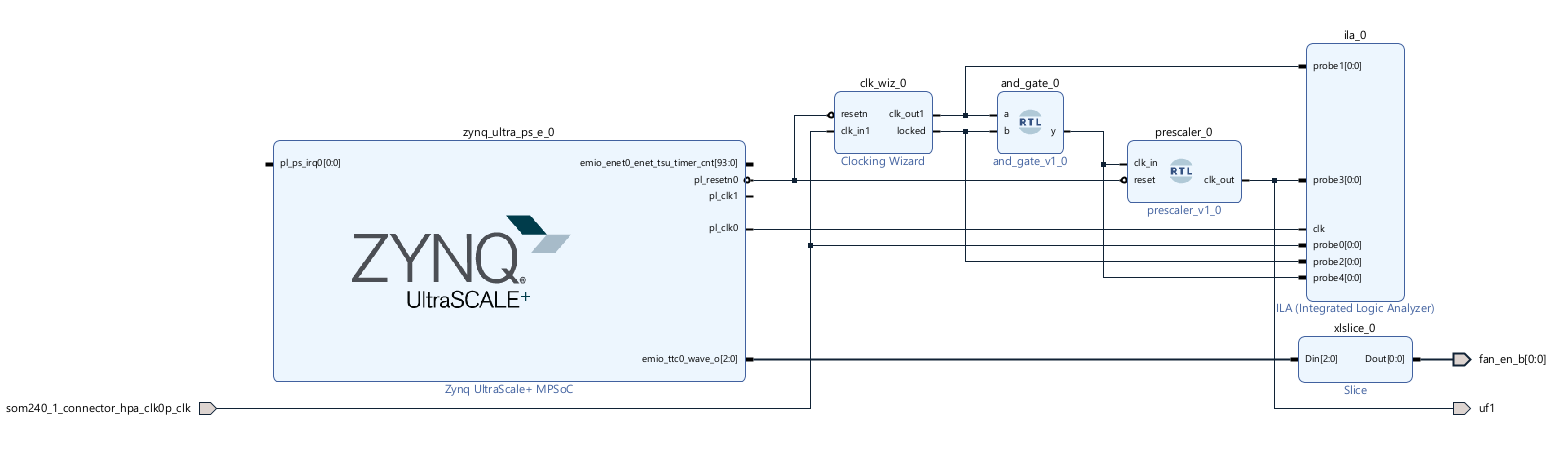
\includegraphics[width=\textwidth]{images/prj3_1}
	\caption{Block Design Layout.}
	\label{fig:prj3_1}
\end{figure} 


\subsection{Block configuration}
The design is composed by few blocks, some of which have already been encountered in the previous implementation. A first, quite useful procedure, is to save the block design of the fan control (example project) and use it as a starting point for new designs. After having opened the fan example, remove both the wrapper and the design file and import the design previously exported (or save the new one with another name). Add and configure the clocking wizard block. Set the reset to be \textbf{active low} and the output clock to be the value that you want (there is, however, a defined range of possible clock frequencies with defined values). For this example the output frequency is set to be $f_{clk-wiz} = 10MHz$. Connect then the and gate, the prescaler and the ILA block as shown in Figure \ref{fig:prj3_1}. Define the output connectors and generate the bitstream. For a more specific configuration, please refer to \href{https://www.hackster.io/LogicTronix/kria-kr260-petalinux-2022-2-gpio-tutorial-9b14bf#toc-vivado-vitis-tool-flow-3}{this page}. Once the bitstream is ready, export the hardware as explained in the previous chapter.




\section{Petalinux project}
The procedure through which the OS is set up and the board booted is the exactly the same defined for the previous project. Also the creation of the bif file and the FPGA programming do not change. Obviously, it will take a while, but at the end the bard will be fully programmed and the led should blink with a frequency of
\begin{equation*}
	f_{blink} = \frac{f_{clk-wiz}}{2 \cdot max\_val} = 10Hz
\end{equation*}



\section{J-TAG debugging}
The main difference between this project and the previous one is the presence of a clock source that will allow for the ILA to trigger and synchronize the displayed signals. After having programmed the FPGA, opened the \textbf{Hardware Manager} and connected the device, Vivado should automatically find the debug-probes file (if not, just re-programm the FPGA). Between the various signals, chose one to be referred as trigger and define the trigger event (equal to a value, rising or falling edge...) and run the trigger event for the ILA core. 
\begin{figure}[ht]
	\centering
	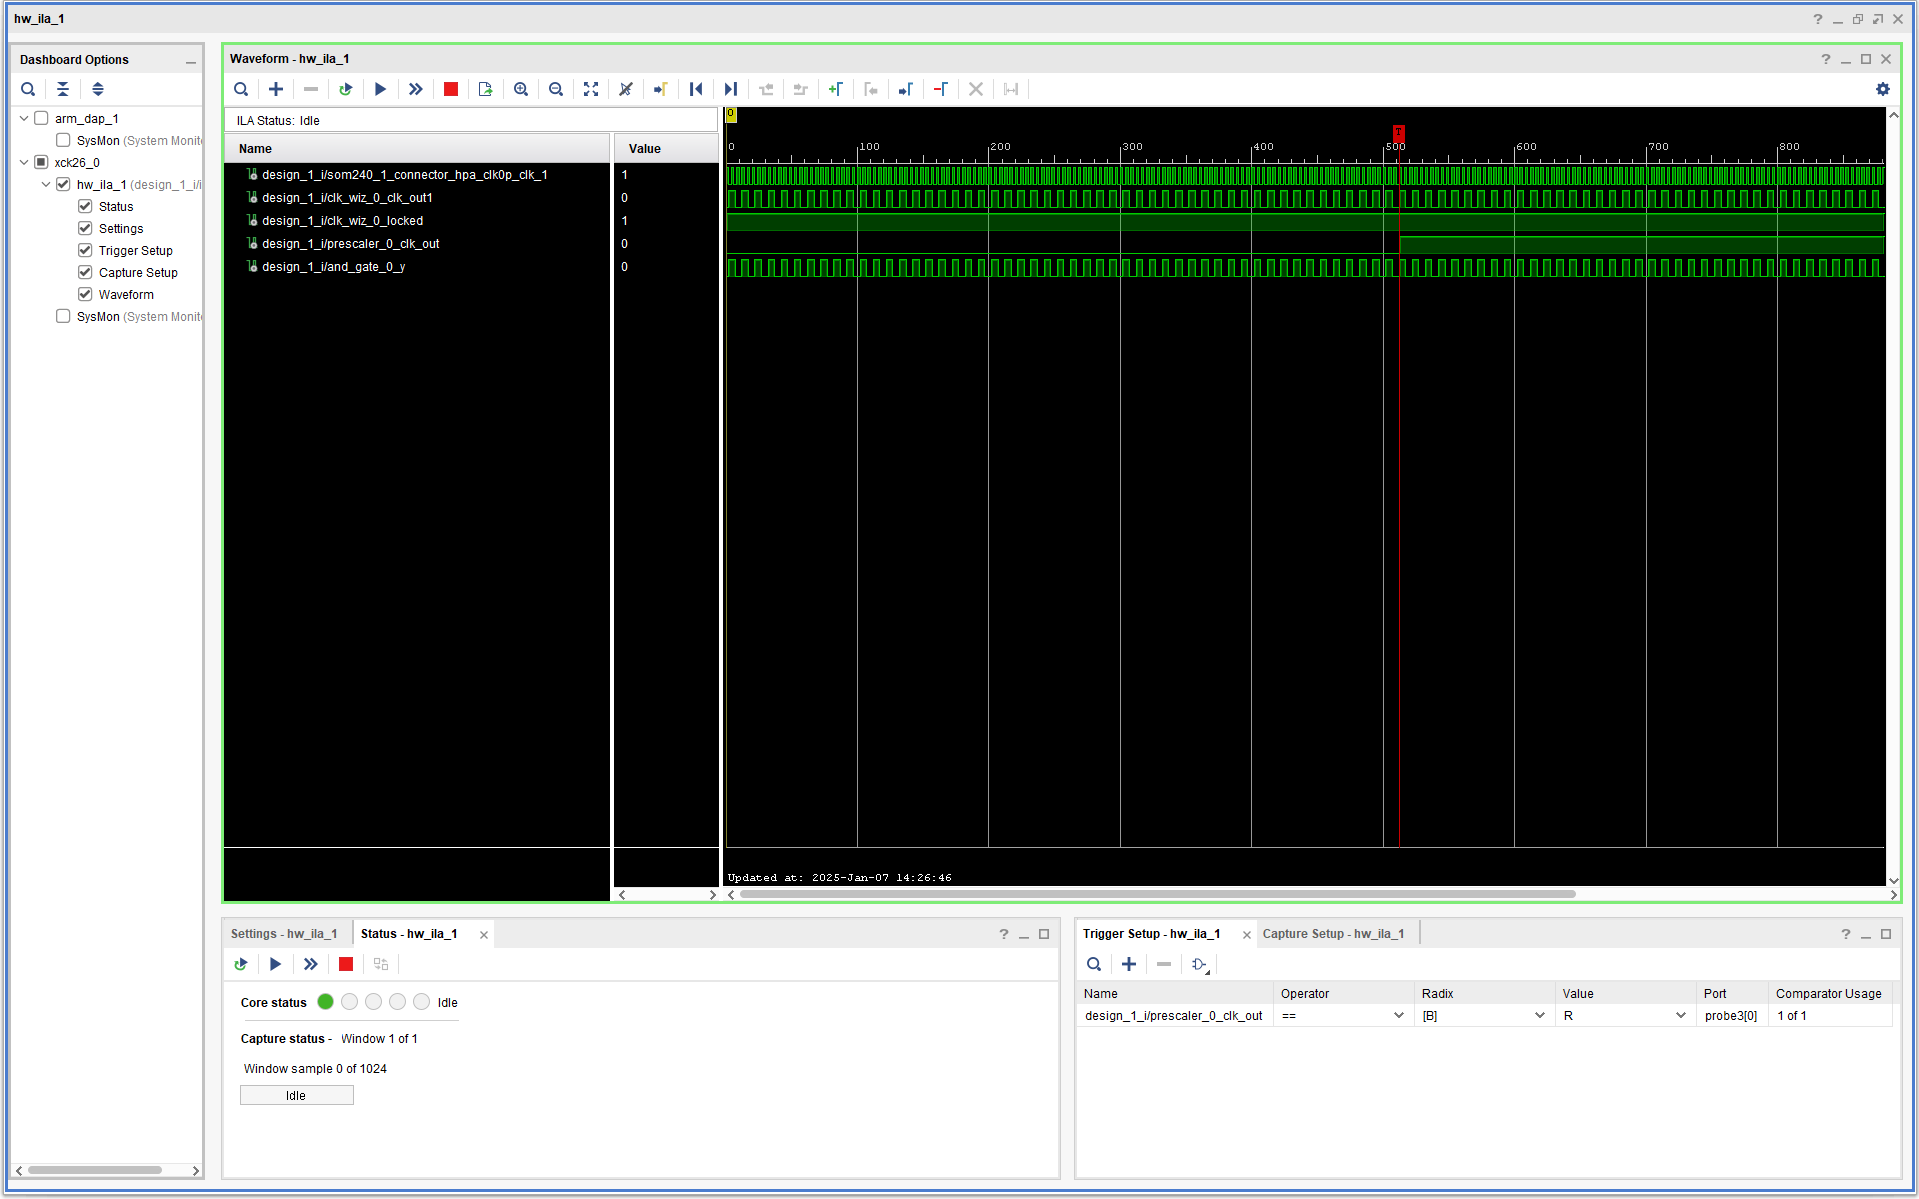
\includegraphics[width=\textwidth]{images/prj3_2}
	\caption{J-Tag debugging with ILA core (triggered on the blinking signal).}
	\label{fig:prj3_2}
\end{figure} 
	\chapter{Project 4: blinking LED with memory access}
So far, the PL and PS parts of the SoM have been exploited separately, without actually interconnecting them so as to control or to communicate with the programmable logic through the system processor. Within this project, more focused is given into the development of design that allows to read a specific memory address in order to communicate with the system processor. To do so, a specific component has been used, which allocate a defined memory address to which R/W operations can be performed.


\section{Vivado project}
Figure \ref{fig:prj4_1} shows the design block scheme of the project. The system processor was set either by applying the procedure linked in the previous chapter or by starting from the fan design example.
\begin{figure}[ht]
	\centering
	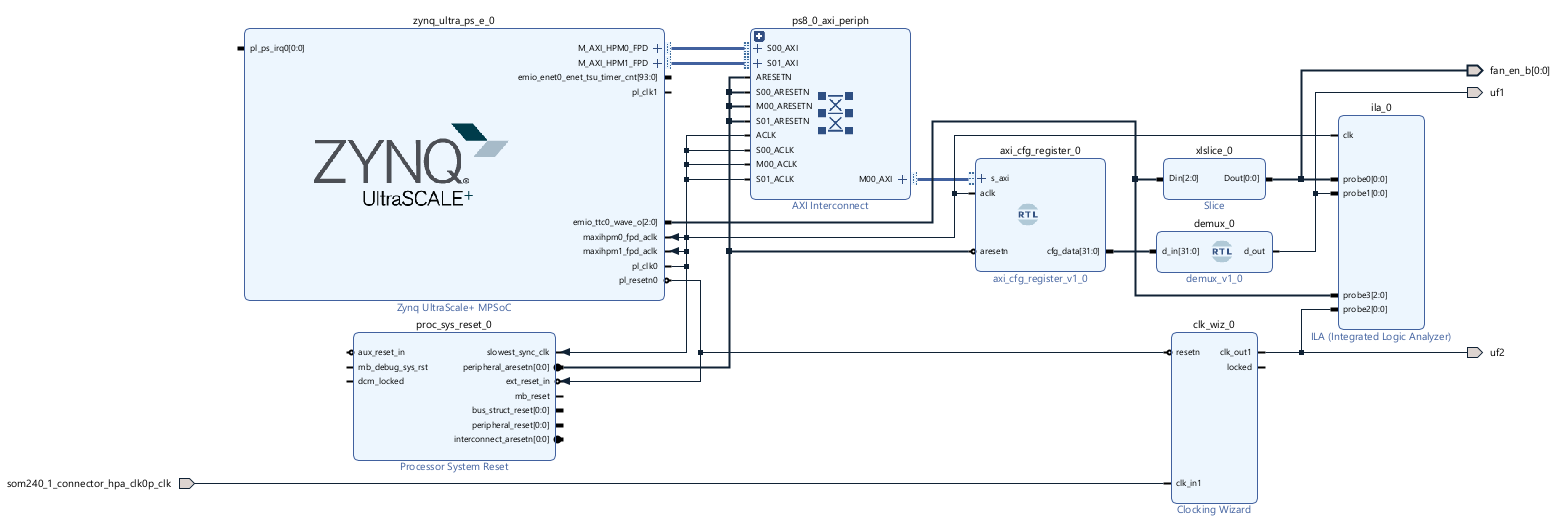
\includegraphics[width=\textwidth]{images/prj4_1}
	\caption{Block Design Layout.}
	\label{fig:prj4_1}
\end{figure} 
From the \textbf{Address Editor} window, the memory space reserved for this application was set to be 128bit (there is no need for higher space, since only a bit is needed to be read and written) and the memory address to $0xB0000000$. 
\begin{figure}[ht]
	\centering
	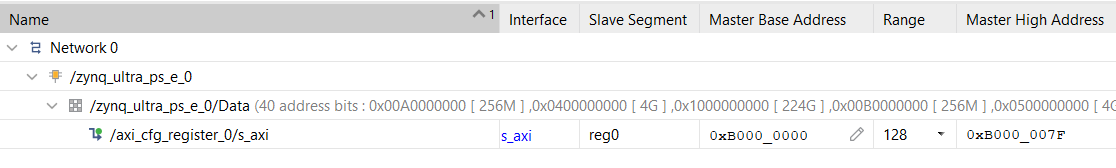
\includegraphics[width=\textwidth]{images/prj4_2}
	\caption{Address editor.}
	\label{fig:prj4_2}
\end{figure}
The component used to perform R/W operations is named \textit{axi\_cfg\_register}. As always, after having generated the bitstream, it is needed to export the hardware including the bitstream with it. Also the creation of the Petalinux project is not different from the previous. What changes is the procedure after the boot of the board.



\section{Code implementation}
After having successfully created and built the project, to perform R/W operations on the memory allocated by the cfg\_register, there is the necessity to define a) the driver and b) the program with which the operations are performed.

\subsection{Driver}
The generation of the driver is beyond the scope of this guide. It is assumed that the corresponding .c and .h files are already available. In this discussion it is explained how to create a driver needed to blink the led, but the same procedure can be applied to a wide variety of applications. Now, assuming the .c and .h files are respectively named 
\begin{verbatim}
	driver_name.c
	driver_name.h
\end{verbatim}
then, the creation of the driver modules is performed with the command
\begin{verbatim}
	petalinux-create -t modules --name driver_name --enable
\end{verbatim}
after which 
\begin{verbatim}
	petalinux-build -c driver_name
\end{verbatim}
will build the module. Now, the aforementioned files .c and .h are to be copied into the \textit{project-spec/meta-user/recipes-modules/driver\_name/files/} path. Finally, to build the module
\begin{verbatim}
	petalinux-build -c driver_name
\end{verbatim}
\subsection{C program}

\section{Board booting}

\section{J-TAG debugging}


	
\end{document}